\chapter{ALI Hardware Components}

The section will list and give specifications for all of the major ALI hardware components. Each section will have a brief description followed by a table of the specifications.

\section{Lenses}

All lenses used in the ALI system were purchased from Newport and were coated with anti-reflective coating AR.16 which covers 650-1000~nm. All the lens in the system were made from N-BK7 glass. The specification and model number of each lens is located in the tabled below.

\begin{table}
    \begin{center}
    \begin{tabular}{|c|c|c|c|}
    \hline
    Model Number & Effective Focal Length (mm) & Diameter (mm) & Type  \\
    \hline
    KPX100AR.16 & 150 & 25.4 & Plano-Convex \\
    \hline
    KPX187AR.16 & 100 & 50.8 & Plano-Convex \\
    \hline
    KBX052AR.16 & 50.2 & 25.4 & Bi-Convex \\
    \hline
    \end{tabular}
    \end{center}
    \caption[ALI System Lenses]{Lenses contained within the ALI system.}
    \label{tab:A.1:AliLenes}
\end{table}

\section{Polarizers}

ALI needed two linear polarizer to help reduce stray light in the system. These polarizers needed a high extinction ratio over the range of the CCD sensitivities to help reduce stray light. The polarizer chosen were model number LPVIS100 from Thor Labs. The extinction ratios and transmission of the device can be seen in \autoref{fig:A.2:LinearPolarizer}.

\begin{figure}
    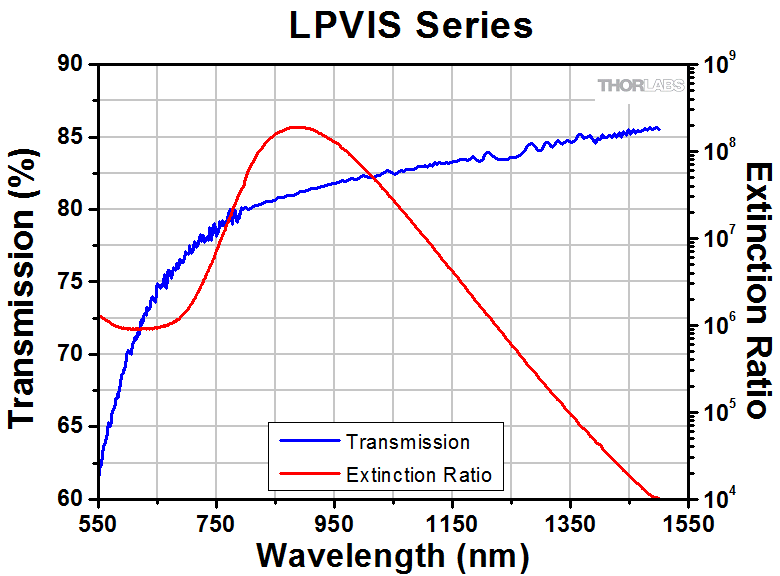
\includegraphics[width=1.0\textwidth]{./Images/A-2-PolarizerExtinctionRatio.png}
    \caption[Linear Polarizer Transmission and Extinction Ratios]{The transmission and extinction ratios of the LPVIS100 used in ALI}
    \label{fig:A.2:LinearPolarizer}
\end{figure}

\section{AOTF}

The AOTF in ALI is made by Brimrose of America and is optically tuned for a range of 600-1200~nm. The following from the following is the specifications of the device. The separation angle is defined the angle between the input source and the desire refracted polarization.

\begin{table}
    \begin{center}
    \begin{tabular}{|l|c|l|c|}
    \hline
    Material & TeO$_{2}$ & Polarization & Linear vertical \\
    \hline
    RF Range (Mhz) & 75-156 & Tunable Range (nm) & 600-1200 \\
    \hline
    Optical Aperture (mm) & 10x10 & Angular Aperture (\si{\degree}) & 5-6 \\
    \hline
    Acceptance Angle(\si{\degree}) & 3 & Separation Angle (\si{\degree}) & 2.7 \\ 
    \hline
    RF Power (W) & 2 & Optical Damage Threshold (W) & 5 \\
    \hline
    \end{tabular}
    \end{center}
    \caption[ALI System Lenses]{Lenses contained within the ALI system.}
    \label{tab:A.1:BrimroseAOTF}
\end{table}

\section{RF Driver}

The driver for ALI is made by Gooch and Housego. It had no internal control mechanism and required additional control hardware to operate the device. In order to pick the frequency a 30-bit digital value is inputed into the device to pick a frequency as well as manage several control line to the device. The control work needed to determine a specific frequency is given by
\begin{equation}
    K_{10} = \frac{F2^{n+1}}{F_{clk}}
\end{equation}
where $K_{10}$ is the 30-bit control work in base 10 rounded to the nearest integer, $F$ is the desired RF to be outputted by the driver, $F_{clk}$ is the internal clock of the driver which is 1000.059~MHz for ALI, and $n$ is the number of bits in the control work for ALI $n=30$. The control word os converted to binary and sent to the device to get the desired RF.

\section{CCD Camera}

The CCD camera was a QSI 616s with a Kodak KAP-1603ME sensor with a mechanical shutter. The spectral response of the device can be seen in \autoref{fig:3.2:QSIQuantumEfficientcy} and generical specification can be seen in \autoref{tab:A.3:QSISpecs}

\begin{table}
    \begin{center}
    \begin{tabular}{|l|c|}
    \hline
    Imager Size (mm) & 13.8 x 9.2 \\
    \hline
    Imager Size & 1536 x 1024 \\
    \hline
    Pixel Size (\si{\micro\meter}) & 9 x 9 \\
    \hline
    Intrinsic Read Noide (eletrons) & 15 RMS \\
    \hline
    Mass (kg) & 0.95 \\
    \hline
    Power Comsumption (W) & 24 \\
    \hline
    Operating Temperature (\si{\degree C}) & -20 to 30 \\
    \hline
    \end{tabular}
    \end{center}
    \caption[QSI 616s Camera Specifications]{QSI 616s Camera Specifications}
    \label{tab:A.3:QSISpecs}
\end{table}

\section{OCELOT Computer}

The on board computer for the ALI instrument was the Ocelot VL-EPMs-21 computer made by VersaLogic. Its architecture is based on the Intel Atom Z5 processor and can have up to 2~GB of DDR2 memory. It has low power draw and fanless operation. It has a temperature range of -40 to 85 \si{\degree C}.
